%%%%%%%%%%%%%%%%%%%%%%%%%%%%%%%%%%%%%%%%%%%%%%%%%%%%%%%%%%%%%%%%%%%%%%
% writeLaTeX Example: Academic Paper Template
%
% Source: http://www.writelatex.com
% 
% Feel free to distribute this example, but please keep the referral
% to writelatex.com
% 
%%%%%%%%%%%%%%%%%%%%%%%%%%%%%%%%%%%%%%%%%%%%%%%%%%%%%%%%%%%%%%%%%%%%%%
% How to use writeLaTeX: 
%
% You edit the source code here on the left, and the preview on the
% right shows you the result within a few seconds.
%
% Bookmark this page and share the URL with your co-authors. They can
% edit at the same time!
%
% You can upload figures, bibliographies, custom classes and
% styles using the files menu.
%
% If you're new to LaTeX, the wikibook is a great place to start:
% http://en.wikibooks.org/wiki/LaTeX
%
%%%%%%%%%%%%%%%%%%%%%%%%%%%%%%%%%%%%%%%%%%%%%%%%%%%%%%%%%%%%%%%%%%%%%%
\documentclass[twocolumn,showpacs,%
  nofootinbib,aps,superscriptaddress,%
  eqsecnum,prd,notitlepage,showkeys,10pt]{revtex4-1}

% displays all math in sans-serif font TODO  
\usepackage[cm]{sfmath}
  
\usepackage{graphicx}
\graphicspath{ {images/} }

\usepackage{listings}
\lstset{
basicstyle=\small\ttfamily,
%basicstyle=\ttfamily,
columns=flexible,
breaklines=true
}
%\lstset{language=Coq}

\usepackage [english]{babel}
\usepackage [autostyle, english = american]{csquotes}
\MakeOuterQuote{"}

\usepackage{amssymb}
\usepackage{amsmath}
\usepackage{graphicx}
\usepackage{dcolumn}
\usepackage{hyperref}

% \newcommand{name}[num]{definition}
\newcommand{\eqn}[1] {\begin{gather*}#1\end{gather*}}
\newcommand{\spc} {\textrm{ }}

\begin{document}

\title{Formally proving equivalence between abstract and concrete specifications of HMAC}
\author{Katherine Ye, advised by Andrew Appel}
\affiliation{Princeton University}

\begin{abstract}
The OpenSSL implementation of HMAC has been proven to correctly implement its concrete specification. HMAC uses SHA-256 as its hash function, and the SHA-256 program has also been proven to correctly implement its specification. At a higher level, HMAC has been proven "safe to use": an abstract specification of HMAC has been proven to be a pseudo-random function given that its internal hash function is one as well. We bridge the gap between the abstract and the concrete HMAC spec by formally proving their equivalence. This proof transfers the desirable and necessary property of being a pseudo-random function (with some caveats) to both the concrete spec and the C implementation of HMAC, guaranteeing that the OpenSSL code is "safe to use."
\\
TODO shorten abstract (December 26, 2014)

\end{abstract}

\maketitle

%%%%%%%%%%%%%%%%%%%%%%%%%%%%%%%%%%%%%%%%%%%%%%%%%

\section{Introduction}

Compelling quote or hook here TODO

There exists a gap between mathematical cryptography (rigorous paper proofs of correctness of an algorithm) and applied cryptography (concrete implementations of those algorithms, plus the field of information security). This gap gives us two reasons to be wary. First, the paper proofs may be flawed, leading us to believe that algorithms are "safe to use" when they are not. (TODO example of wrong crypto proof) Second, even if the proofs are right, they are accompanied by a specification of the algorithm only on paper. The concrete code implementing this specification may contain exploitable bugs, allowing hackers to induce buffer overflows, ... TODO (TODO OpenSSL, Heartbleed) 

Recent work aims to close this gap. Barthe (2013, 2014) assert that "cryptographic proofs have become essentially unverifiable," and present CertiCrypt, a framework that "enables the machine-checked
construction and verification of code-based proofs." This paper continues in the spirit of formal verification. 

At a high level, this work is motivated by two purposes. First, the Verified Software Toolchain project has built the framework to do TODO, and HMAC is a natural extension of the existing SHA-256 work. See Appel 2015 for an explanation of the system. Second, encrypted communications between military robots requires HMAC TODO. 

Toward this end, we

The rest of this paper assumes introductory knowledge of cryptography and and no knowledge about proof assistants or formal verification.

\begin{figure}[h!]
	\centering
	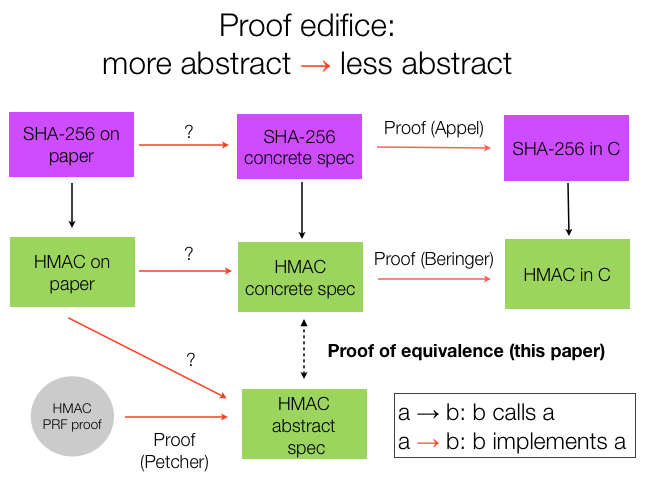
\includegraphics[scale=0.35]{Proof_edifice}
	\caption{Mind the gap (the dotted arrow).}
\end{figure}	

\subsection{Formal verification in Coq}

Coq is a proof assistant.

Coq has two internal languages, Gallina and the tactic language. Gallina is a purely functional language similar to OCaml. The tactic language is used for doing proofs and defining new proof strategies.

As used here, formal verification of a piece of code means proving that this implementation fulfills some kind of high-level specification. The code will usually be written in a low-level language such as C and may contain optimizations and other tricks. The specification, or "spec," will usually be written in a high-level language such as OCaml or Gallina and is typically more mathematical and abstract. As Appel 2015 notes, "A program without a specification {\it cannot be incorrect}, it can only
be surprising."

For example, TODO sorting algorithm

TODO: insert diagram of what formal verification means

Coq has been used to

\subsection{The Merkle-Damgard construction}
% TODO add accent on Damgard
Say we have a strong cryptographic compression function TODO define. It has certain guarantees. However, it only operates on an input of a fixed length.

The Merkle-Damgard construction (referred to as "M-D" from now on) is a way to extend this function to inputs of any length by iterating the compression function on identically-sized, adjacent blocks of the input. It has been proven to uphold the desirable properties of C such as

\begin{figure}[h!]
	\centering
	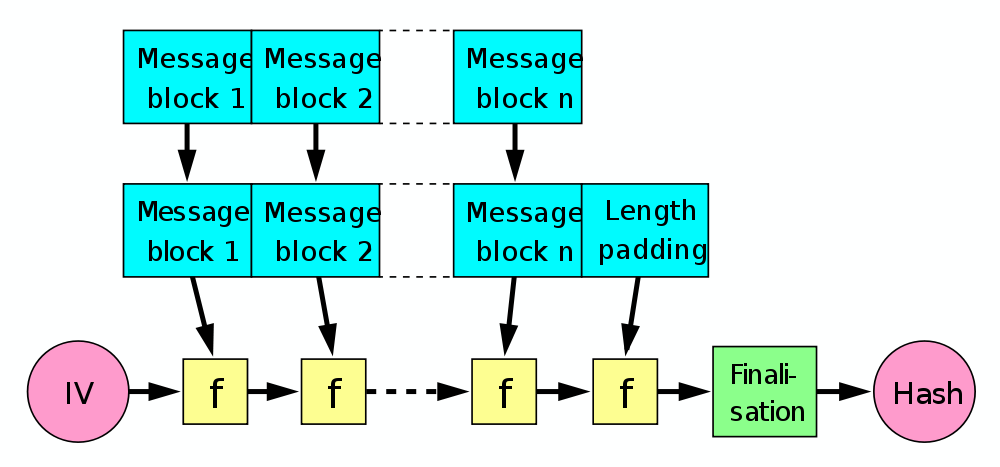
\includegraphics[scale=0.24]{Merkle-Damgard}
	\caption{The M-D construction.}
\end{figure}

SHA-256 is an example of an application of M-D.

Picture of crypto system 

\subsection{SHA-256}

SHA-256 is a cryptographic hash algorithm used for TODO. Mention OpenSSL.

It operates on a message of any length by breaking the message into 512-bit blocks. TODO (is this right?) It outputs a 256-bit digest. 

Like all such hash functions, it comes with guarantees of pre-image resistance, second pre-image resistance, and collision resistance. Thus, it is very difficult for an adversary to change the input message without changing the digest.

Inner hash function

PRF

\subsection{HMAC}

SHA-256 provides only a guarantee of integrity; that is, a guarantee the message has not been tampered with. A message authentication code (MAC) is used to guarantee both integrity and authenticity, the latter meaning that the message's origin is the expected sender. Sender and receiver need only exchange a secret key before beginning their communication. In addition, whereas SHA-256 is vulnerable to length-extension attacks, HMAC is not.

To accomplish this, HMAC (a "hash-based message authentication code") was designed in Bellare 1996. It includes a proof that the HMAC protocol (described below) is a pseudo-random function (PRF) on its inputs given that the underlying hash primitive is a PRF. In SHA-256, the underlying hash primitive would be its compression function.
% TODO different MAC security requirements

To compute the authentication code of a message, RFC 2104 defines HMAC as the following action:
$$HMAC_{H, K}(m) = H ( (k \oplus opad) | H ( k \oplus ipad | m )  ) $$

where

\begin{itemize}
\item its block length is 512 bits, or 64 bytes,
\item $H$ is a cryptographic hash function (here, $SHA$-$256$),
\item $K$ is a secret key padded to the right with extra zeros to the input block size of the hash function, or the hash of the original key if it's longer than that block size, 
\item $m$ is the message to be authenticated, 
\item $|$ denotes concatenation, 
\item $\oplus$ denotes bitwise exclusive or (XOR), 
\item $opad$ is the outer padding (the byte $0x5c$ repeated 64 times to be the length of one block), 
\item and $ipad$ is the inner padding ($0x36$ repeated as above).
\end{itemize}

Note that formalizing HMAC is a natural extension of our work on SHA-256, since HMAC is not much more complicated than applying a cryptographic hash function twice. 

OpenSSL includes an implementation of HMAC in C which calls the OpenSSL implementation of SHA-256.

\begin{figure}[h!]
	\centering
	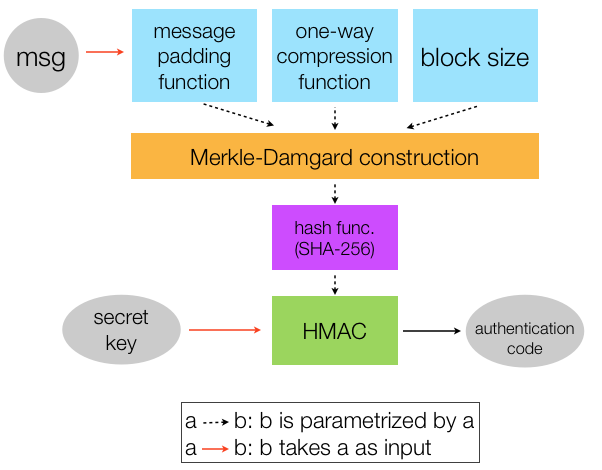
\includegraphics[scale=0.4]{Cryptosystem}
	\caption{The entire system. It is slightly more correct to think of a "black box" HMAC taking message and key as input, and outputting the authentication code.}
\end{figure}

\subsection{Prior work}

Verification of SHA-256.

%%%%%%%%%%%%%%%%%%%%%%%%%%%%%%%%%%%%%%%%%%%%%%%%%

\section{The proof of equivalence}

\subsection{The concrete HMAC spec}

This spec was written to conform to RFC 2104; thus, it contains runnable code, operates on byte lists, and returns a byte list. The spec distinguishes between the $Z$ type and the $byte$ type (values of type $Z$ in range $[0, 256)$); however, we will use $Z$ synonymously with $byte$ with the understanding that all values are in range.

The spec is constructed to work with generic cryptographic hash functions. We will instantiate it with the $SHA$-$256$ functional program, which we treat as a black box that takes care of the message padding and compression function iteration.

The code for this spec and the next is in the Appendix.

\subsection{The abstract HMAC spec}

% TODO elaborate on Bellare stuff
This spec was written to conform to the HMAC protocol defined in Bellare 1996; thus, to be as general as possible, it operates on bit vectors and returns a bit vector. (A bit vector $Bvector \textrm{ } n$ is a type dependent on a natural number value $n$, the length of the vector.)

It defines HMAC via the two-keyed HMAC ($HMAC\_2K$) and generalized HMAC ($GHMAC\_2K$) structures, rather than straightforwardly as the concrete spec does. It also includes an implementation of generalized NMAC ($GNMAC$), another structure used in the proof.

The spec does not contain runnable code as-is because it leaves several parameters abstract:

\lstinputlisting[lastline=19]{../HMAC_spec_parameters.v}

% TODO code here

The proof depends on the following assumptions that are explicit in the spec:
\begin{enumerate}
\item the key is of the right length (one block)
\item $opad \neq ipad$ (they differ in at least one bit)
\item the padding function $splitAndPad$ is one-to-one
\item the hash function (e.g. $SHA$-$256$) is an iterated version of the compression function, a la Merkle-Damgard.
\end{enumerate}

as well as other implicit assumptions explained in Section III.

The fourth assumption can be seen in this definition of the $SHA$-$256$ analogue, $hash\_words$:

\lstinputlisting[firstline=23, lastline=28]{../HMAC_spec_parameters.v}

However, $SHA$-$256$ includes a padding function for the message, while this spec's use of dependent types ($Bvector \textrm{ } n$) forces the use of two types of ad-hoc padding, the functions $app\_fpad$ and $splitAndPad$.

\lstinputlisting[firstline=55, lastline=59]{../HMAC_spec_abstract.v}

\subsection{Proof outline}

Equivalence of specs means 

\begin{figure}[h!]
	\centering
	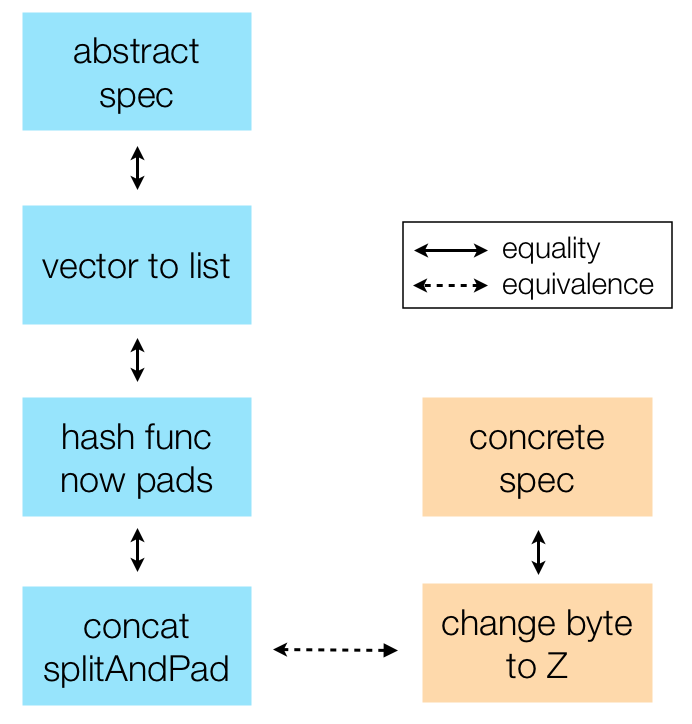
\includegraphics[scale=0.56]{Equivalence_proof_chain}
	\caption{Stages of the equivalence/equality proofs.}
\end{figure}

Again, the main differences between the specs are that (TODO make a table)
\begin{enumerate} 
\item GNMAC and GHMAC\_2K structures
\item the abstract spec operates on bits, whereas the concrete spec operates on bytes
\item the abstract spec uses the dependent type \verb|Bvector n|, which is a bit list of length $n$, whereas the concrete spec uses byte lists and int lists
\item the abstract spec pads its input twice in an ad-hoc manner, whereas the concrete spec uses the SHA-256 padding function consistently
\item the SHA-256 concrete spec uses the Z type, whereas the HMAC concrete type uses the byte type, which is Z constrained to be in $[0, 255]$.
\end{enumerate}

We solve some of them by massaging the two specs in the "same direction."

%%%%%
\subsection{Bridging bytes and bits}

We would like to prove that the concrete and abstract HMAC specs ($HMAC_c$ and $HMAC_a$) are extensionally equal. That is, equal inputs always result in equal outputs: 
\begin{gather*}
k_c = k_a \rightarrow \\
m_c = m_a \rightarrow \\
HMAC_c(k_c, m_c) = HMAC_a(k_a, m_a).
\end{gather*}

However, $HMAC_c$ operates on bits (in fact, vectors of bits) and $HMAC_a$ operates on bytes (lists of bytes). So the statement $k_c = k_a$ (for example) does not have meaning because the types are different. To solve this, we generalize equality to equivalence. Given that the inputs are {\it equivalent}, the outputs will be {\it equivalent}.
\begin{gather*}
k_c \approx  k_a \rightarrow \\
m_c \approx m_a \rightarrow \\
HMAC_c(k_c, m_c) \approx HMAC_a(k_a, m_a).
\end{gather*}

The equivalence relation $\approx$ can be defined either computationally or inductively. Both definitions will turn out to be useful. (From now on, we will use $b$ to name a value of type $Blist$ (list of booleans, or bits) and $B$ to name a value of type $list$ $Z$ (list of bytes).)

The computational relation is 
\begin{gather*}
b \approx_c B := \\
b = bytesToBits \textrm{ } B,
\end{gather*} where $bytesToBits : list \textrm{} Z \rightarrow Blist$ is a conversion function.

% TODO explain inductive
The inductive relation is 
\begin{gather*}
b \approx_i B := \\
bytes\_bits\_lists \textrm{ } b \textrm{ } B.
\end{gather*}

where $bytes\_bits\_lists : Blist \rightarrow list \textrm{ } Z \rightarrow Prop$ creates an "assertion" that $b$ and $B$ are related in this way, together with two constructors used to provide evidence to prove the assertion. (For more on inductively defined propositions, see the $Prop$ chapter in the Coq textbook "Software Foundations.")

% TODO fix formatting
\lstinputlisting[firstline=27, lastline=34]{../ByteBitRelations.v}

The inductive and computational definitions have been proven equivalent in the sense that 
$$bytes\_bits\_lists \textrm{ } b \textrm{ } B \leftrightarrow b = bytesToBits \textrm{ } B.$$

For several other ways to convert between the definitions, see $ByteBitRelations.v$.

% Insert abstract section here

\subsection{Instantiating the abstract specification}

We instantiate the block sizes and wrap the concrete functions in $byteToBit$ and/or $intlist\_to\_Zlist$ conversion functions. The latter is necessary because portions of the $SHA$-$256$ spec operate on lists of $Integer$s (four bytes, or $Z$, combined into 32 bits), as specified in FIPS Pub. 180-2.

\lstinputlisting[firstline=32, lastline=48]{../HMAC_spec_parameters.v}

Note that we are essentially converting the type of the values from $intlist \rightarrow \ldots \rightarrow intlist$ to $Blist \ldots \rightarrow \ldots Blist$ by converting their inputs and outputs.

We can use the computational equivalence relation defined earlier ($\approx_c$), instantiated with a generic conversion function, to reason abstractly about the behavior of such wrapped functions. Let's define the framework as such (letting $. = \circ$, function composition):

\lstinputlisting[firstline=52, lastline=58]{../HMAC_spec_parameters.v}

Note that the types $B$ and $A$ are not symmetric, in the sense that 

Define two relations as such:
\eqn{
x \approx_c X := \\
x = convert\_BA \textrm{ } X.
}
\eqn{
f \approx_w F := \\
f = wrap \textrm{ } F.
}

We ask: what assumptions are needed such that application of equivalent (via wrapping) functions to equivalent (via conversion) inputs result in equivalent (via conversion) outputs?
\eqn{
Lemma \spc once\_eq : \\
\forall \spc (x : A) \spc (X : B) \spc (f : A \rightarrow A) \spc (F : B \rightarrow B),\\
x \approx_c X \rightarrow \\
f \approx_w F \rightarrow \\
f \spc x \approx_c F \spc X
}

The necessary and sufficient assumption (together with the other two assumptions) is that we have output equivalence exactly when a "round-trip" of composing the two conversion functions results in the identity function. (The reader is invited to write out this short proof.)
\eqn{
Lemma \spc roundtrip : convert\_AB \circ convert\_BA = id }

Indeed, we have proven that $bitsToBytes \circ bytesToBits = id$. Note that it does not hold the other way around. $bytesToBits \circ bitsToBytes$ is false if the length of the bit list input is not a multiple of 8.

A natural extension is to prove output equivalence on repeated application of the wrapped functions, or iteration:

\lstinputlisting[firstline=78, lastline=82]{../HMAC_spec_parameters.v}

\eqn{
Lemma \spc iterate\_equiv : \\
  \forall  \spc (x : A) \spc (X : B)\\
   (f : A \rightarrow A) \spc (F : B \rightarrow B) \spc (n : nat), \\
    x \approx_c X \rightarrow \\
    f \approx_w F \rightarrow \\
    iterate \spc n \spc f \spc x = convert\_BA \spc (iterate \spc n \spc F \spc X).
}

Here we need both $once\_eq$ and our newly admitted assumption $roundtrip$, which can be rephrased as $\forall (X : B), X = roundtrip \spc X$. The proof is completed by induction on $n$.

This framework is not just an academic exercise. $once\_equiv$ and $iterate\_equiv$ correspond directly to several lemmas in the bytes/bits equivalence proof.

In particular, $iterate\_equiv$ corresponds to the SHA-256 operation of hashing blocks. % TODO code here

Round-trip and conversion properties. Galois connections or other algebraic structure?

This is the usefulness of the computational definition.

\subsection{Main lemmas}

Now, the usefulness of the inductive definition

It allows us to break it up into 4 main lemmas: main proof

\subsection{Other proof techniques}

The following techniques may be useful in future equivalence proofs.

\begin{itemize}
\item Many theorems are true for lists of any length (e.g. some involving map and zip). We found it difficult to do dependent type induction. Instead, we found it easy to prove theorems by induction on a Blist, implying that the list may be any length, then specialize it to \verb|Bvector n|, a Blist of length $n$. 
\item Likewise, we found it easier to prove theorems about lists of any length (or a certain length given by an assumption), then prove that the functions involved preserve the length. This is equivalent to working with \verb|Bvector n|.
\item When dealing with lists whose lengths must be a multiple of a block size (e.g. 512 bits or 64 bytes), we found it useful to define an inductive proposition \verb|InWords n l| that would allow one to do proofs by inducting in the block size, cons'ing elements to the front. We then proved this equivalent to the computational version (using the length function).
\item Likewise, we found it useful to define two things: a function to compute conversions between byte lists and bit lists, and an inductive proposition stating that the lists correspond in this way.
\item When it comes to theorems that involve tricky math, we exploited the fact that range of a byte is $[0, 255]$ and proved them by brute force instead. The same technique also works in reverse. Proving something true for $8$ booleans is as simple as checking that the statement is true for each of the $256$ cases.
\end{itemize}

\subsection{Problems encountered}

\begin{itemize}
\item We found it difficult to work with dependent types, induction, and John Major equality.
\item We encountered problems converting between many machine representations: byte/Z, byte/bit, int/Z, and even little-endian vs. big-endian.
\item We did not find much prior work on this sort of equivalence proof, except for related functions in Coq.Strings.Ascii.
\end{itemize}

\section{The proof of HMAC's safety}

\subsection{The 1996 (?) Bellare proof}

Let $f$ be the compression function and $f^*$ the iteration of $f$.

Given the assumption that $f$ is a pseudo-random function (PRF), that implies that $f^*$ is computationally almost universal ($cAU$). $cAU$ is a slightly weaker property than collision-resistant.

% (\verb|goo.gl/wK8OXg|)
\begin{figure}[h!]
	\centering
	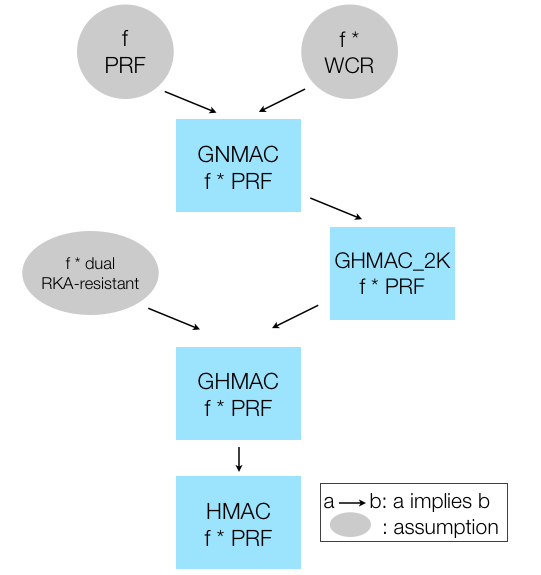
\includegraphics[scale=0.4]{HMAC_proof}
	\caption{The structure of the 1996 (? TODO) Bellare HMAC proof.}
\end{figure}

The $f^* cAU$ property is used to prove that generalized NMAC (GNMAC) using $f^*$ is a PRF. The GNMAC property is used to prove that generalized HMAC with two keys (\verb|GHMAC_2k|) using $f^*$ is a PRF.

Using that fact and the assumption that $f^*$ is RkA-resistant (?), we prove that GHMAC (single-keyed) using $f^*$ is a PRF. This, plus the fact that the padding function for $f$ is one-to-one, leads finally to the proof that HMAC using $f^*$ is a PRF.

%%%%%%%%%%%%%%%%%%%%%%%%%%%%%%%%%%%%%%%%%%%%%%%%%

\subsection{Formalization in Coq}

See Adam Petcher's paper on MCF. Random oracles, monadic syntax.

\subsection{Transfer of properties}

In order for the the proof to hold, the following assumptions must be true:
\begin{itemize}
\item the padding function (which? TODO) is one-to-one
\item opad and ipad differ in at least one bit.
\item (anything else? TODO)
\end{itemize}

Examining the final spec, these are true. TODO

Thus, the property TODO transfers. (termination and well-definedness of C code? Adam's email?)

Interfaces that drop out of the proof are TODO, leaving an end-to-end proof of correctness.

\section{conclusion}

Contribution to cryptography: bridging the gap between concrete and abstract HMAC specs allows the desirable property of being a PRF to transfer to the OpenSSL implementation of HMAC. So it's "safe to use."

Contribution to reasoning about equivalence: many bytes/bits computational and inductive definitions. Lemmas for correspondence between them. 

Contribution to proof techniques: results of trying to use dependent types. Brute force. Inductive propositions for length, plus InBlocks correspondence with division, mod, and existence.

\subsection{Future work}

Dependent types, type-level programming in Coq.

Libraries could be written to aid reasoning about equivalence and lengths.

More crypto formalization! EasyCrypt, CertiCrypt, IMDEA. MCF

SHA PRF, of course

How to transmit HMAC key? Need RSA. Work being done at Princeton.


\begin{acknowledgments}

Andrew Appel, Lennart Beringer, Adam Petcher, and Qinxiang Cao.

\end{acknowledgments}

\section{references}

RFC 2104 (HMAC, 1997): \\
\verb|https://tools.ietf.org/html/rfc2104|

FIPS Publication 180-4 (Secure Hash Standard, containing SHA-256): \\
\verb|http://csrc.nist.gov/publications/PubsFIPS.html|

"Verification of SHA-256," Appel 2015

"New Proofs for NMAC and HMAC: Security without Collision-Resistance," Bellare (1996)

"Keying Hash Functions for Message Authentication," Bellare (2004)

"MCF," Petcher (unpublished)

Barthe 2009

"Merkle-Damgard in EasyCrypt," IMDEA

"Certified Programming with Dependent Types," Chlipala

"Software Foundations," Pierce et al.

"Verified Functional Algorithms," Appel, OPLSS

"HMAC" Wikipedia page

"SHA-256" Wikipedia page

Coq.Strings.Ascii

OpenSSL HMAC and SHA-256 code

%%%%%%%%%%%%%%%%%%%%%%%%%%%%%%%%%%%%%%%%%%%%%%%%%

\section{appendix}

% TODO syntax highlighting and nicer font
\subsection{The abstract HMAC spec}

\lstinputlisting{../HMAC_spec_abstract.v}

\subsection{The concrete HMAC spec}

\lstinputlisting[lastline=90]{../HMAC_functional_prog.v}

\subsection{Definitions}

\lstinputlisting[firstline=173, lastline=190]{../HMAC_spec_harvard_concat.v}

\lstinputlisting[firstline=20, lastline=24]{../ByteBitRelations.v}

\lstinputlisting[firstline=27, lastline=34]{../ByteBitRelations.v}

\subsection{The equivalence proof}

\lstinputlisting[firstline=858]{../HMAC_spec_harvard_concat.v}

\subsection{Selected theorems and proofs}

See the repository at \\ \verb|github.com/hypotext/vst-crypto|.

\end{document}